This thesis set out to create a parametric L-system capable of representing complex plant-left structures. And to use the L-system to procedurally generate plant-life with all of the relavant information necessary for physical simulation. This chapter will first test several features of the parametric L-system such as varying branch width and branching angles, to produce different effects within the plant-life. To test the physical simulation of the L-system there are several different examples which are all running the same physics simulation, with the acceleration due to gravity being kept at a constant value of $9.8m/s^2$. 

The parametric L-system below contains a number of variables that considerably change the visual properties of the tree. The next few examples will illustrate how changing these parameters can not only effect the look of the plant but also how it reacts in a physical simulation. The table shows two sets of default values that will be applied to the L-system. Each example will change the values of one or two of these parameters and show its effect on the plants structure or how it reacts in the simulation.

\vspace{10mm}
\hrule
\begin{singlespace}
\begin{equation}
\begin{aligned}
	&\textrm{\#object F BRANCH;}\\
	&\textrm{\#w : !(1.4)F(2.0, scstart)/(45)A(scstart);}\\
	&\textrm{\#p1 : A(sc) : * : !(dr)F(2, sc)[\&(a3)F(2, sc)A(sc)]/(a1)[\&(a3)F(2, sc)A(sc)]/(a2)[\&(a3)F(2, sc)A(sc)];}\\
	&\textrm{\#p2 : F(l, sc) : * : F(l*dl, sc*scmod);}\\
	&\textrm{\#p3 : !(w) : * : !(w*dr);}
\end{aligned}
\end{equation}
\end{singlespace}

\begin{table}[h!]
\centering
\begin{tabular}{ | c | c | c | c | c | c | c | c | c | }
\hline
	Variation Name & n & a1 & a2 & a3 & dl & dr & scstart & scmod\\  
\hline
\hline
	L-system 1  & 6 & 112.5 & 157.5 & 22.5 & 1.1 & 1.4 & 200 & 1.0 \\
\hline
	L-system 2  & 6 & 137.5 & 137.5 & 18.95 & 1.1 & 1.2 & 200 & 1.0 \\
\hline
	L-system 3  & 7 & 112.5 & 157.5 & 22.5 & 1.1 & 1.4 & 200 & 1.0 \\
\hline
\end{tabular}
\caption{Table of turtle graphics instructions symbols and their meaning to the interpreter}
\label{DOL-system instructions}
\end{table}
\FloatBarrier
\hrule

\vspace{10mm} 

\noindent
In the example in figure \ref{example thickness}, the value `dr', manipulates how thick each branch is. It does this during the rewriting process. Every time the width module `!' is encountered, it is rewritten with the current width multiplied by the value of `dr', which increases the width exponentially each time it is rewritten. This relationship can be expressed as $r_{i+1} = r_i \times dr$, where $r_i$ is the current branch radius and $r_{i+1}$ is the radius of the branch in the next generation. This gives a tree that gets thinner exponentially. For a tree that gets thinner linearly the relationship can be expressed as $r_{i+1} = r_i + dr$. This can be shown in the graphs in figure \ref{graph thickness} below. 

Although this example is not a physical simulation, it could be simulated. Due to the larger width of the branches near the base of the tree, they would have a higher mass and therefore have more inertia, making them more resistant to changes in velocity.

\begin{figure}[htbp]
	{\centering
		\vspace{7px}
		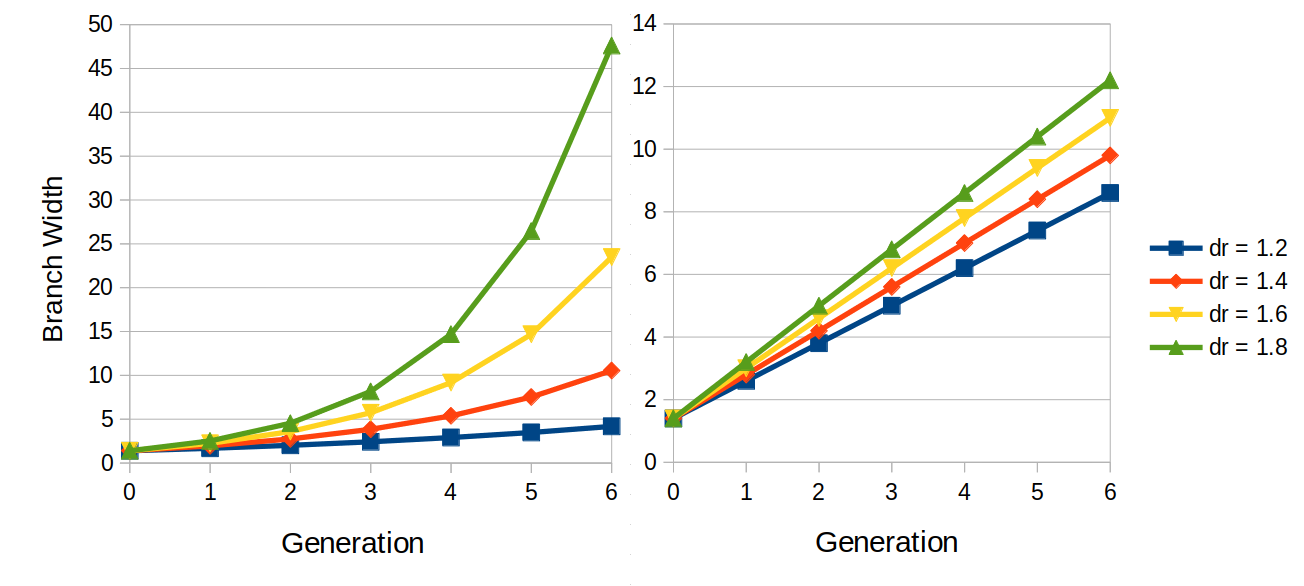
\includegraphics[scale=0.35]{Diagrams/branchWidthIncrease.png}
		\caption{Graph showing an exponential and linear relationship between the branch width and the generation when increasing the value of `dr'.} \label{graph thickness}
	}
\end{figure}
\FloatBarrier

\begin{figure}[htbp]
	{\centering
		\vspace{7px}
		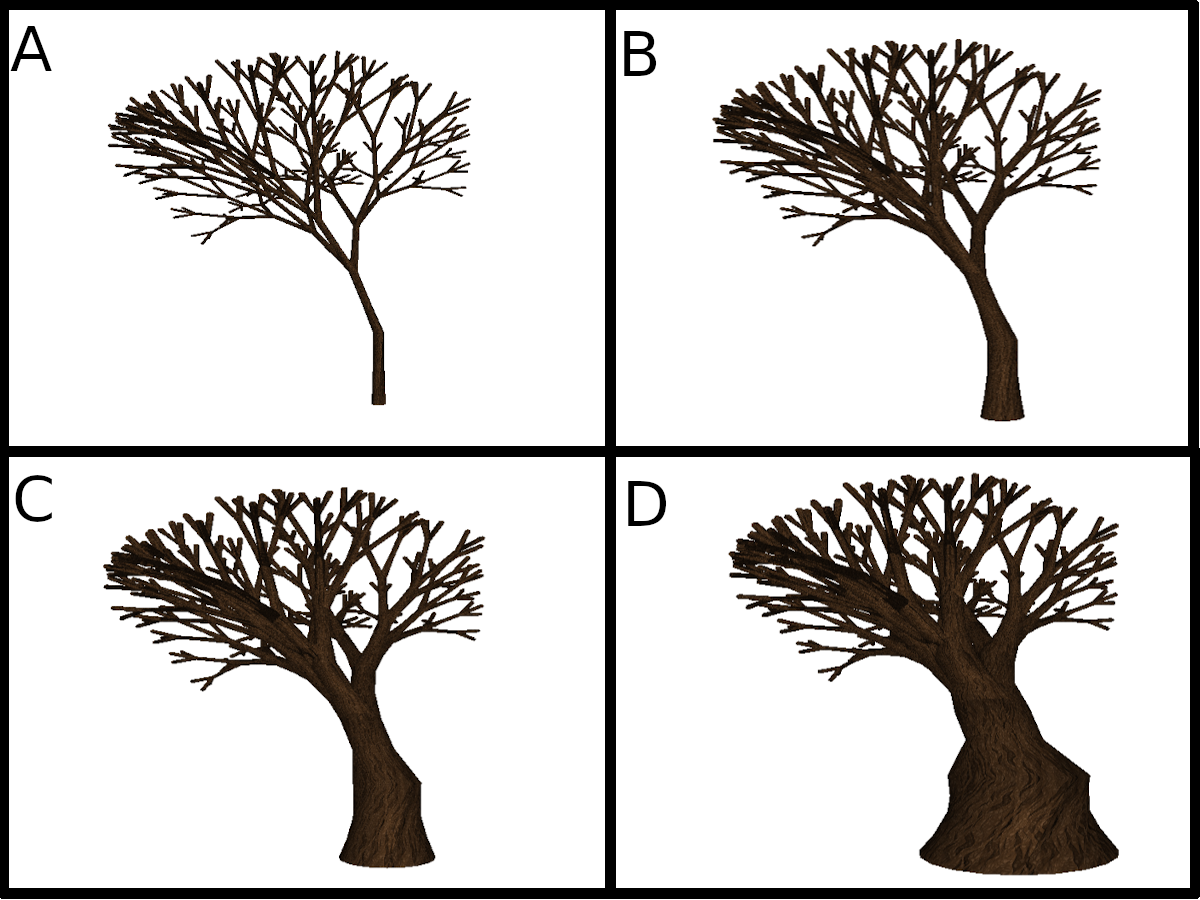
\includegraphics[scale=0.25]{Diagrams/TernaryBranching3_vr.png} 
		\caption{Examples of L-system 1 changing the `dr' variable which modifies the thickness of the base of the tree.} \label{example thickness}
	}
\end{figure}
\FloatBarrier

\noindent
The figure \ref{example angle} below shows that the result of changing the roll rotations' angle for some of the branches gives the tree a very different shape. In this case, increasing the angle of the branches' roll rotation can create a branch that curles slightly. Increasing this angle causes a more dramatic result. Furthermore, the angles of rotations can be randomised using the random range feature to create a tree with branches that are more erratic. 

\begin{figure}[htbp]
	{\centering
		\vspace{7px}
		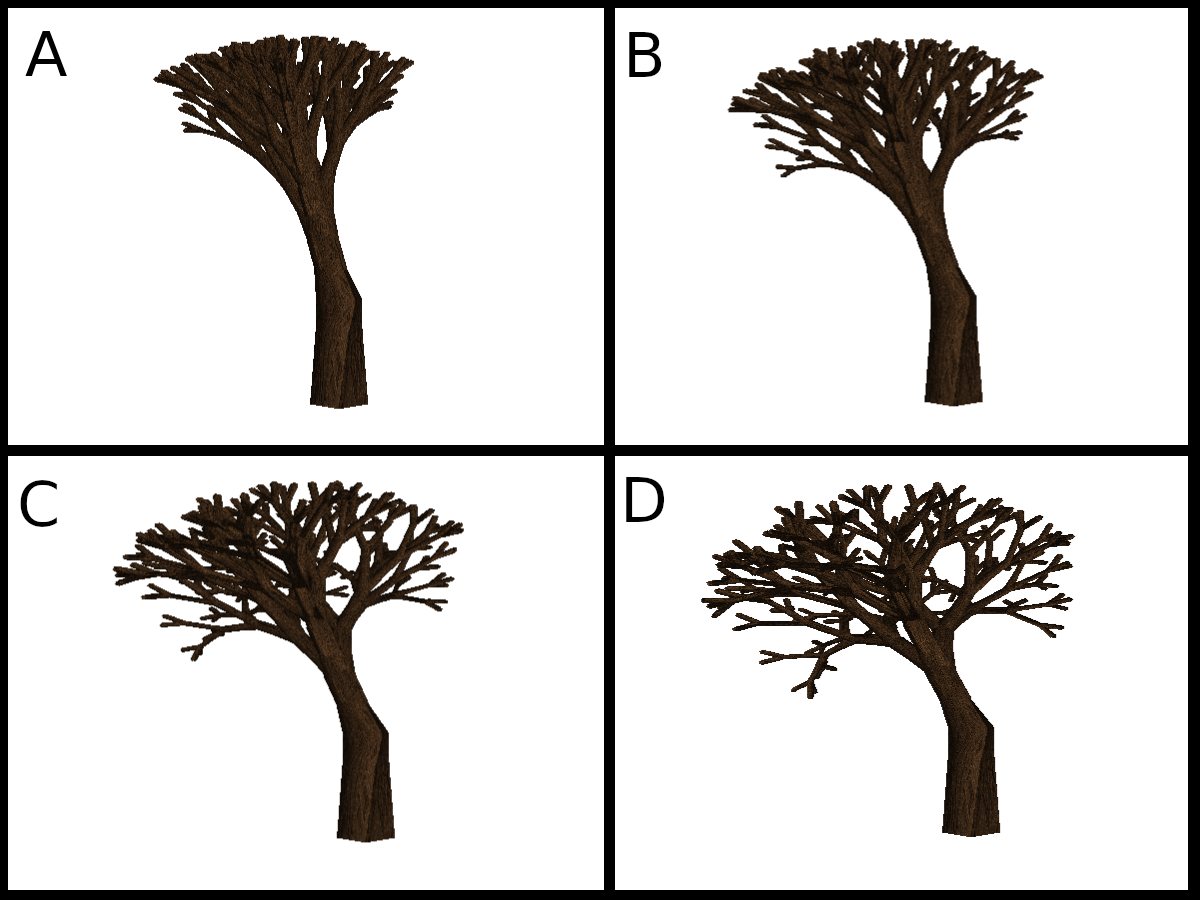
\includegraphics[scale=0.25]{Diagrams/TernaryBranching2_angle_example.png}
		\caption{Examples of L-system 2 changing the `a3' variable modifying the roll angle of certain branches.} \label{example angle}
	}
\end{figure}
\FloatBarrier


\begin{singlespace}
\begin{equation}
\begin{aligned}
	&\textrm{\#n = 6;} \\
	&\textrm{\#define r 20; \#define d 0.4; \#define w 0.5;}\\
	&\textrm{\#w : !(w)Z;}\\
	&\textrm{\#p1 : Z : * : F(d, 30.0)[-(r)Z]F(d, 30.0)[+(r)Z]-(r)Z;}\\
	&\textrm{\#p2 : F(s, x) : * : F(s, x)F(s, x);}
\end{aligned}
\end{equation}
\end{singlespace}

\begin{figure}[htbp]
	{\centering
		\vspace{7px}
		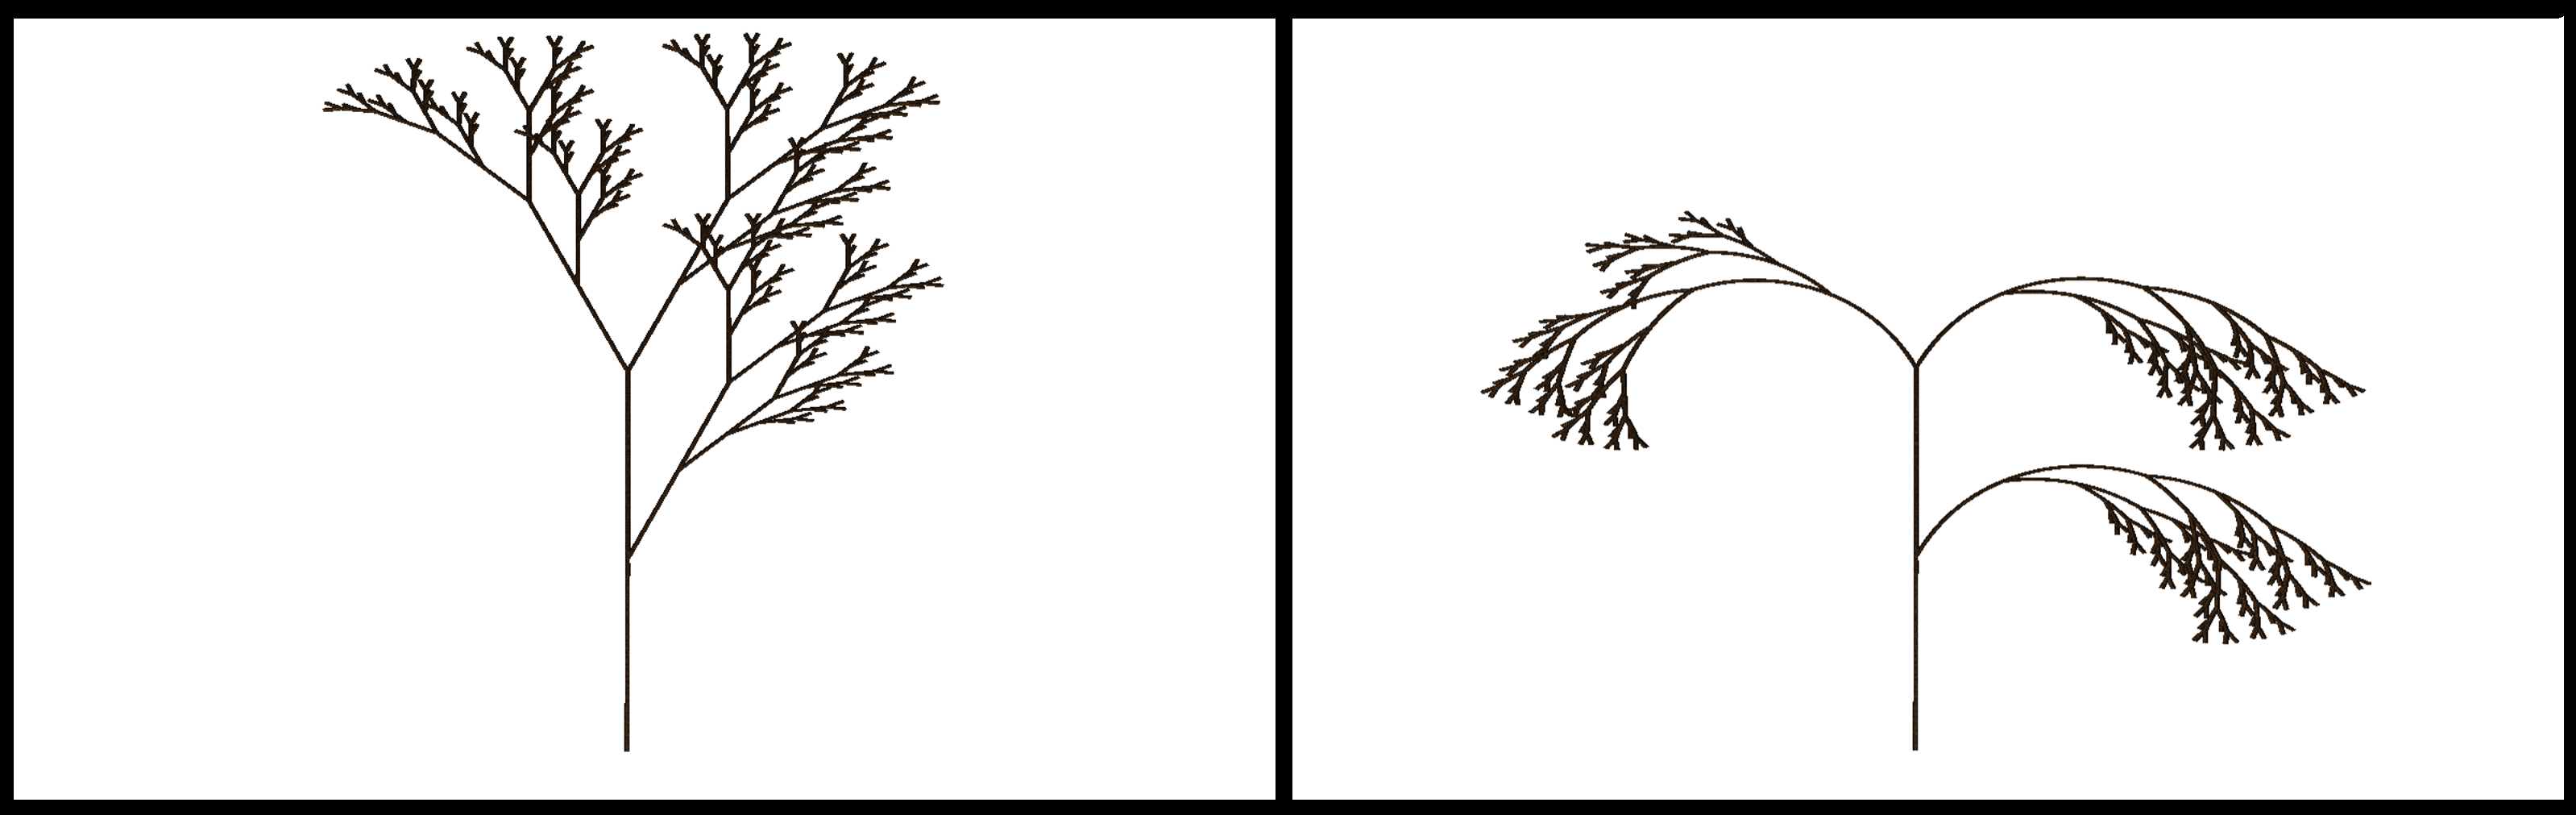
\includegraphics[scale=0.1]{Diagrams/gravityExamples1.png}
		\label{3DAxisFigure} \label{Gravity applied to generated models}
		\caption{Examples simulating gravity on a 2D model}
	}
\end{figure}
\FloatBarrier

\noindent
The L-system above is a 2D fractal tree that has rendered in three dimensions. It is a 2D tree as it only consists of left and right yaw rotations signified with the `+ and -' symbols without any pitch or roll rotations. In this tree, the rotation `r' is defined as 20$^{\circ}$, the distance `d' is 0.4, and the width `w' is 0.5. The spring constant of the branches is kept at a constant 30.0. This means that all the branches are equally prone to bending. 

\begin{singlespace}
\begin{equation}
\begin{aligned}
	&\textrm{\#n = 5;} \\
	&\textrm{\#object F BRANCH; \#object X SPHERE;}\\
	&\textrm{\#define r 25.7; \#define d 0.5; \#define w 1;}\\
	&\textrm{\#define scstart 30; \#define scmod 1.0;}\\
	&\textrm{\#w : !(1.707)X;}\\
	&\textrm{\#p1 : X : * : F(d, scstart)[!(w)/(r)+(r)X][!(w)-(r)X][!(w)$\land$(r)X][!(w)\&(r)X]!(w)F(d, scstart)X;}\\
	&\textrm{\#p2 : F(s, x) : * : F(s, x * scmod)F(s, x * scmod);}
\end{aligned}
\end{equation}
\end{singlespace}

\begin{figure}[htbp]
	{\centering
		\vspace{7px}
		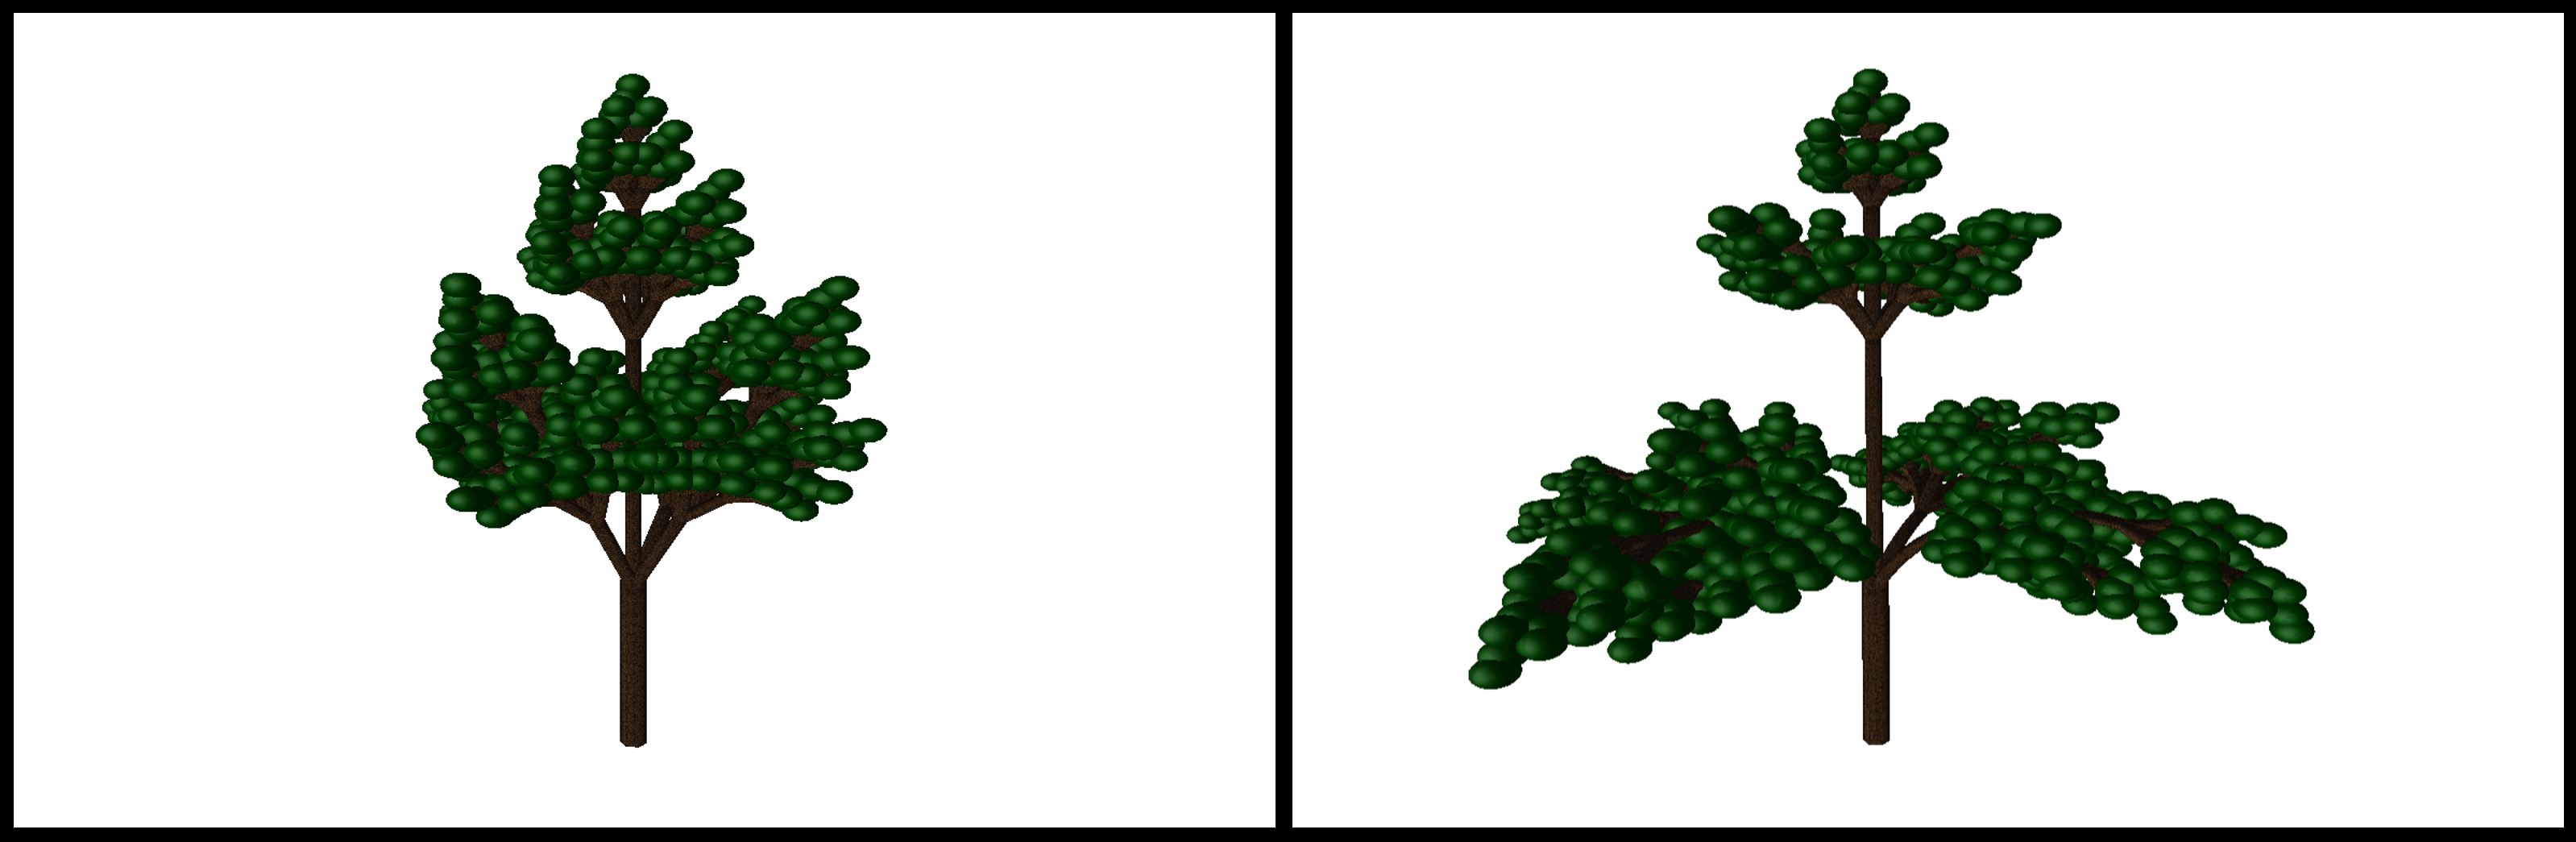
\includegraphics[scale=0.1]{Diagrams/gravityExamples2.png}
		\label{3DAxisFigure} \label{Gravity applied to generated models}
		\caption{Examples simulating gravity on a 3D model}
	}
\end{figure}
\FloatBarrier



\begin{figure}[htbp]
	{\centering
		\vspace{7px}
		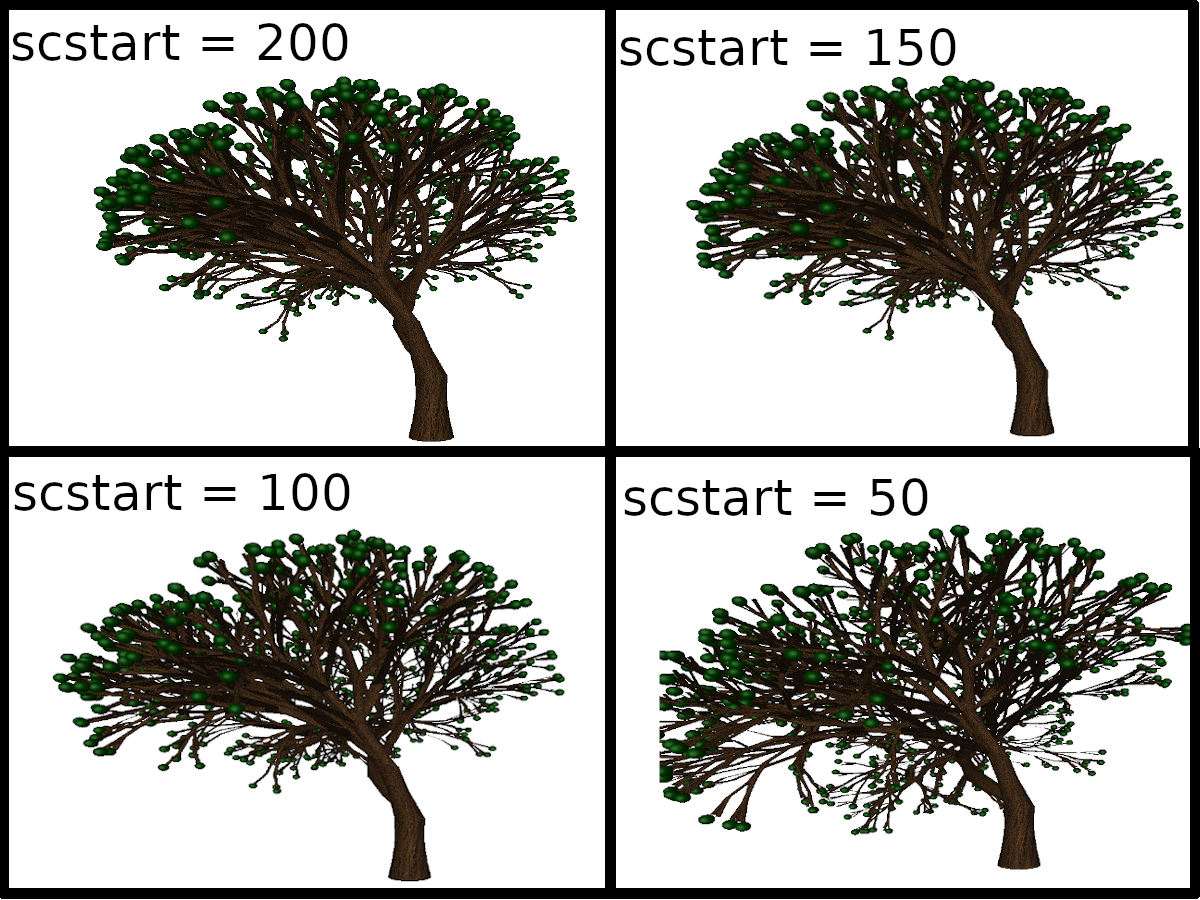
\includegraphics[scale=0.25]{Diagrams/TernaryBranching3_constantSC.png}
		\caption{Examples of L-system 1 with gravity applied when uniformly changing the spring constant `scstart' for all branches.}
	}
\end{figure}
\FloatBarrier

\noindent
In the previous simulations above the spring constant variable `scstart' has been a constant value throughout all of the branches. This makes the assumption that a thick branch near the base of the tree is as bendy as a thin branch at the top of the tree. This is not accurate and will result in large branches bending unrealistically. Similarly to the example for modifying the width of branches, a similar method can be used the increase the spring constant for branches closer to the base of the tree, leaving branches near the top of the tree to have the weekest spring constant. The rate at which the spring constant increases is determined by the spring constant modifier `scmod'. 

\begin{figure}[htbp]
	{\centering
		\vspace{7px}
		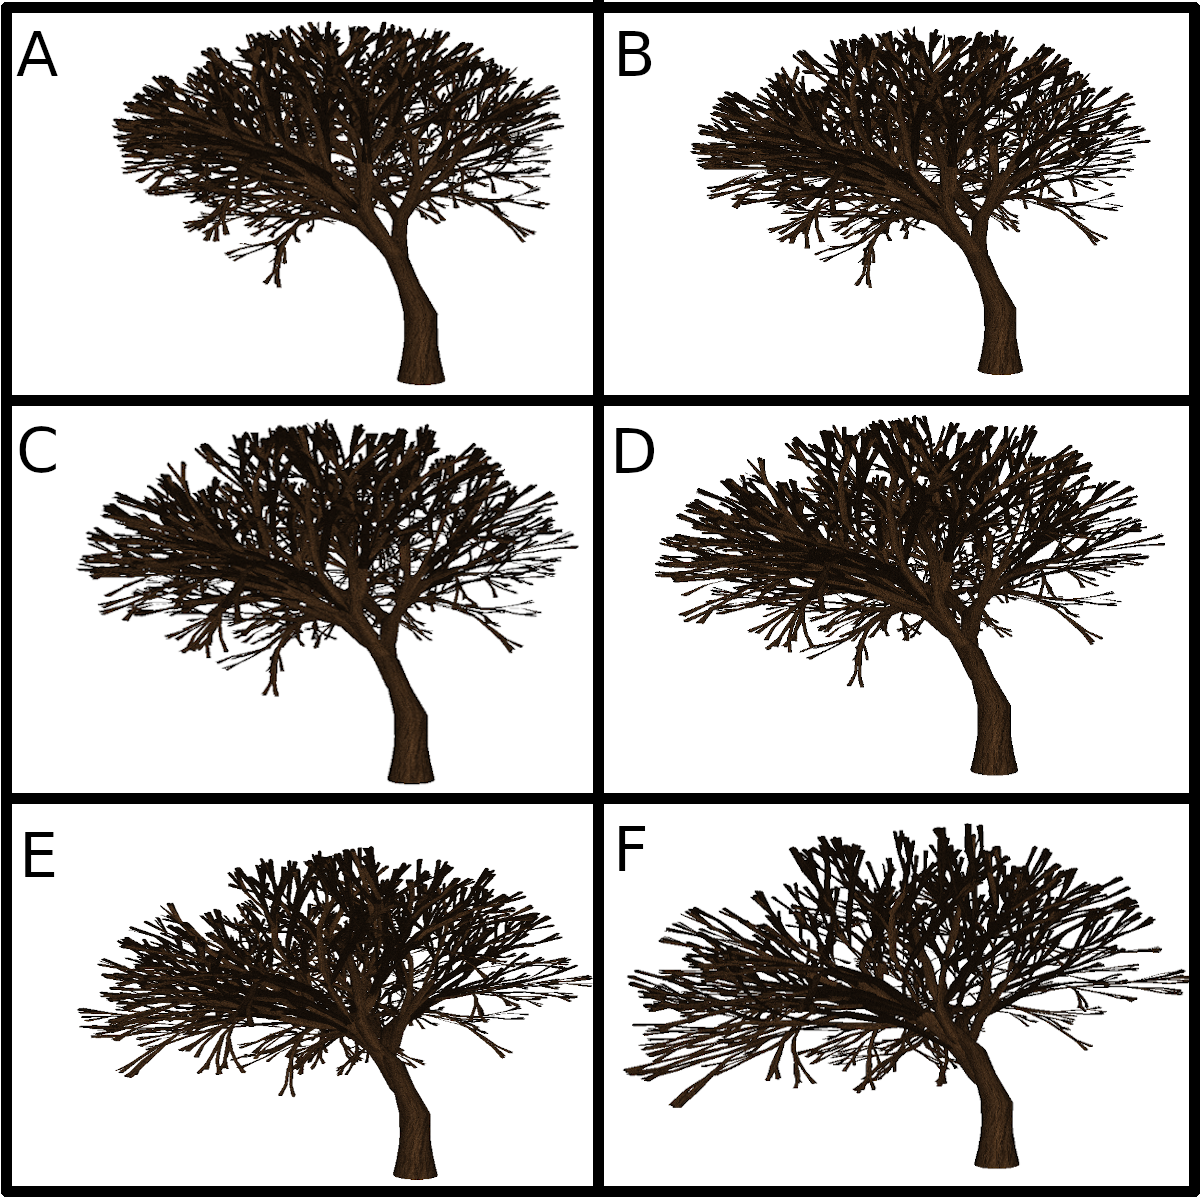
\includegraphics[scale=0.25]{Diagrams/TernaryBranching3_scmod.png}
		\caption{Examples of L-system 3 with gravity applied when changing the spring constant modifier `scmod', when the starting spring constant is set to 30 `scstart = 30'.}
	}
\end{figure}
\FloatBarrier



